\usepackage{xcolor}
\usepackage{afterpage}
\usepackage{pifont,mdframed}
\usepackage[bottom]{footmisc}

\makeatletter
\gdef\this@inputfilename{input.txt}
\gdef\this@outputfilename{output.txt}
\makeatother

\newcommand{\inputfile}{\texttt{input.txt}}
\newcommand{\outputfile}{\texttt{output.txt}}

\newenvironment{warning}
  {\par\begin{mdframed}[linewidth=2pt,linecolor=gray]%
    \begin{list}{}{\leftmargin=1cm
                   \labelwidth=\leftmargin}\item[\Large\ding{43}]}
  {\end{list}\end{mdframed}\par}

	When commuting by train, Italian people tend to just sit in the first empty seat they find instead of spending time looking for their reserved seat. Specifically: when an Italian person boards a train, he/she will start looking for an empty seat (from the very first seat in the train) and they will stop only:

    \begin{itemize}
        \item When an empty seat is encountered: in this case, that person will occupy the seat. Or...
        \item When the actual seat, reserved to that person, is encountered: in this case, if the seat is occupied, the person will kindly ask the offending traveler to move. The offending traveler will apologize, get up, and go to their reserved seat (\emph{not} just some empty seat, this time).
    \end{itemize}

    Note that, in the second case presented, a \emph{chain reaction} of movings could fire up (\emph{A} asks \emph{B} to move, then \emph{B} asks \emph{C} to move, and so on).

    \begin{figure}[H]
        \centering
        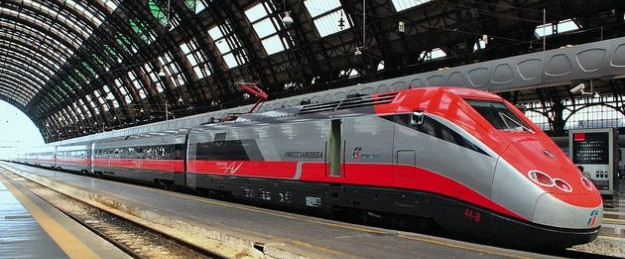
\includegraphics[width=0.9\linewidth]{treno.jpg}
        \caption{A \emph{Frecciarossa} train in the \emph{Milano Centrale} station.}
    \end{figure}

    Train seats are numbered from $0$ to $N-1$. Every person who boards the train will start looking for an empty seat from the $0$-th seat (the ``head'' of the train), and then walk up to the $(N-1)$-th seat (the ``tail'' of the train).

    Giorgio loves travelling by train. Today, sitting in his reserved seat, he has seen a lot of travelers boarding/leaving, moving around the train, asking other travelers to get up. Since Giorgio hates when his reserved place is occupied, he wanted to measure how bad the Italian situation really is and started wondering: how many people, in total, had to get up and apologize to other travelers?

    You have the list of ``events'' that Giorgio witnessed (from the train departure to its arrival), which can be either ``a person, for which the $k$-th seat was reserved, \emph{boards} the train'' or ``a person, for which the $k$-th seat was reserved, \emph{leaves} the train''. Compute how many times a person had to get up and give their seat to another passenger.

\begin{warning}
Among the attachments of this task you may find a template file \texttt{seats.*} with a sample incomplete implementation.
\end{warning}

\InputFile
The first line contains two integers $N$ and $Q$, the number of seats in the train and the number of events, respectively.

Other $Q$ lines follow, each containing a character $T_i$ representing the type of event (\texttt{`b'} for ``boards the train'', \texttt{`l'} for ``leaves the train''), and an integer $K_i$ representing the seat \emph{reserved to the person} in this event (not necessarily the seat they actually sat on).

\OutputFile
You need to write a single line with an integer: how many times someone had to apologize and get up.

% Assunzioni
\Constraints
\begin{itemize}[nolistsep, itemsep=2mm]
	\item $1 \le N, Q \le 100\,000$.
	\item $T_i$ is either `\texttt{b}' or `\texttt{l}' for each $i=0\ldots Q-1$.
	\item $0 \le K_i \le N - 1$ for each $i=0\ldots Q-1$.
	\item The events are consistent (e.g. the same person won't board the train twice, and it won't happen that a non-existent person leaves the train).
    \item After a person leaves the train, a new person with the same reserved seat could board the train.
\end{itemize}

\Scoring
Your program will be tested against several test cases grouped in subtasks.
In order to obtain the score of a subtask, your program needs to correctly solve all of its test cases.

\begin{itemize}[nolistsep,itemsep=2mm]
  \item \textbf{\makebox[2cm][l]{Subtask 1} [\phantom{1}0 points]}: Examples.
  \item \textbf{\makebox[2cm][l]{Subtask 2} [10 points]}: $N, Q \le 10$.
  \item \textbf{\makebox[2cm][l]{Subtask 3} [20 points]}: $N, Q \le 1000$.
  \item \textbf{\makebox[2cm][l]{Subtask 4} [70 points]}: No additional limitations.
\end{itemize}

% Esempi

\Examples
\begin{example}
\exmpfile{seats.input0.txt}{seats.output0.txt}%
\exmpfile{seats.input1.txt}{seats.output1.txt}%
\end{example}

\Explanation
In the \textbf{first sample case} three people board the train in the following manner:

{
\color{gray}  \verb|    A >> |  \color{black}  \verb| ___ ==> A__| \\
\color{gray}  \verb|    B >> |  \color{black}  \verb| A__ ==> AB_| \\
\color{gray}  \verb|    C >> |  \color{black}  \verb| AB_ ==> CB_|  \color{red}  \verb| (A)| \\
\color{gray}  \verb|    A -> |  \color{black}  \verb| CB_ ==> CA_|  \color{red}  \verb| (B)| \\
\color{gray}  \verb|    B -> |  \color{black}  \verb| CA_ ==> CAB| \\
}

In the \textbf{second sample case}, five people board the the train and one leaves it:

{
\color{gray}  \verb|    A >> |  \color{black}  \verb| ____ ==> A___| \\
\color{gray}  \verb|    B >> |  \color{black}  \verb| A___ ==> AB__| \\
\color{gray}  \verb|    C -> |  \color{black}  \verb| AB__ ==> CB__|  \color{red}  \verb| (A)| \\
\color{gray}  \verb|    A -> |  \color{black}  \verb| CB__ ==> CA__|  \color{red}  \verb| (B)| \\
\color{gray}  \verb|    B -> |  \color{black}  \verb| CA__ ==> CAB_| \\
\color{gray}  \verb|         |  \color{black}  \verb| CAB_ ==> _AB_|  \color{gray}  \verb|  ~> C| \\
\color{gray}  \verb|    D >> |  \color{black}  \verb| _AB_ ==> DAB_| \\
\color{gray}  \verb|    E -> |  \color{black}  \verb| DAB_ ==> EAB_|  \color{red}  \verb| (D)| \\
\color{gray}  \verb|    D -> |  \color{black}  \verb| EAB_ ==> EABD| \\
}
